% Options for packages loaded elsewhere
\PassOptionsToPackage{unicode}{hyperref}
\PassOptionsToPackage{hyphens}{url}
%
\documentclass[
]{article}
\usepackage{amsmath,amssymb}
\usepackage{iftex}
\ifPDFTeX
  \usepackage[T1]{fontenc}
  \usepackage[utf8]{inputenc}
  \usepackage{textcomp} % provide euro and other symbols
\else % if luatex or xetex
  \usepackage{unicode-math} % this also loads fontspec
  \defaultfontfeatures{Scale=MatchLowercase}
  \defaultfontfeatures[\rmfamily]{Ligatures=TeX,Scale=1}
\fi
\usepackage{lmodern}
\ifPDFTeX\else
  % xetex/luatex font selection
\fi
% Use upquote if available, for straight quotes in verbatim environments
\IfFileExists{upquote.sty}{\usepackage{upquote}}{}
\IfFileExists{microtype.sty}{% use microtype if available
  \usepackage[]{microtype}
  \UseMicrotypeSet[protrusion]{basicmath} % disable protrusion for tt fonts
}{}
\makeatletter
\@ifundefined{KOMAClassName}{% if non-KOMA class
  \IfFileExists{parskip.sty}{%
    \usepackage{parskip}
  }{% else
    \setlength{\parindent}{0pt}
    \setlength{\parskip}{6pt plus 2pt minus 1pt}}
}{% if KOMA class
  \KOMAoptions{parskip=half}}
\makeatother
\usepackage{xcolor}
\usepackage{graphicx}
\makeatletter
\def\maxwidth{\ifdim\Gin@nat@width>\linewidth\linewidth\else\Gin@nat@width\fi}
\def\maxheight{\ifdim\Gin@nat@height>\textheight\textheight\else\Gin@nat@height\fi}
\makeatother
% Scale images if necessary, so that they will not overflow the page
% margins by default, and it is still possible to overwrite the defaults
% using explicit options in \includegraphics[width, height, ...]{}
\setkeys{Gin}{width=\maxwidth,height=\maxheight,keepaspectratio}
% Set default figure placement to htbp
\makeatletter
\def\fps@figure{htbp}
\makeatother
\setlength{\emergencystretch}{3em} % prevent overfull lines
\providecommand{\tightlist}{%
  \setlength{\itemsep}{0pt}\setlength{\parskip}{0pt}}
\setcounter{secnumdepth}{-\maxdimen} % remove section numbering
\ifLuaTeX
  \usepackage{selnolig}  % disable illegal ligatures
\fi
\IfFileExists{bookmark.sty}{\usepackage{bookmark}}{\usepackage{hyperref}}
\IfFileExists{xurl.sty}{\usepackage{xurl}}{} % add URL line breaks if available
\urlstyle{same}
\hypersetup{
  hidelinks,
  pdfcreator={LaTeX via pandoc}}

\author{}
\date{}

\begin{document}

\section{Intro}\label{intro}

\subsubsection{v.0.1}\label{v.0.1}

This is a \textbf{VEGETARIAN and GLUTENFREE Cookbook} for
cyclingtravelers and other long-term travelers who dont like to cook.

When we embarked on our journey of cycling the world, I had little
knowledge about cooking. In fact, neither my partner nor I were fan of
spending time in the kitchen, and leaving our normie lifestyle behind
was part of the appeal of this trip.

Both my partner and I follow a strict gluten-free diet\footnote{Gluten-free,
  especialy wheat-free nuriture prevents us from having depressions!}.
During our travels, we both became vegetarian. Our encounters with
animals and witnessing the realities of large-scale meat production
factories made consuming meat feel ethically wrong and groce. While
everyone has their own preferences, please note that there won't be any
recipes featuring products of dead animals.

No more dirty kitchen, you are going to cook on very different places
with a lot of new challenges\ldots{}

\newpage

\section{Impressions}\label{impressions}

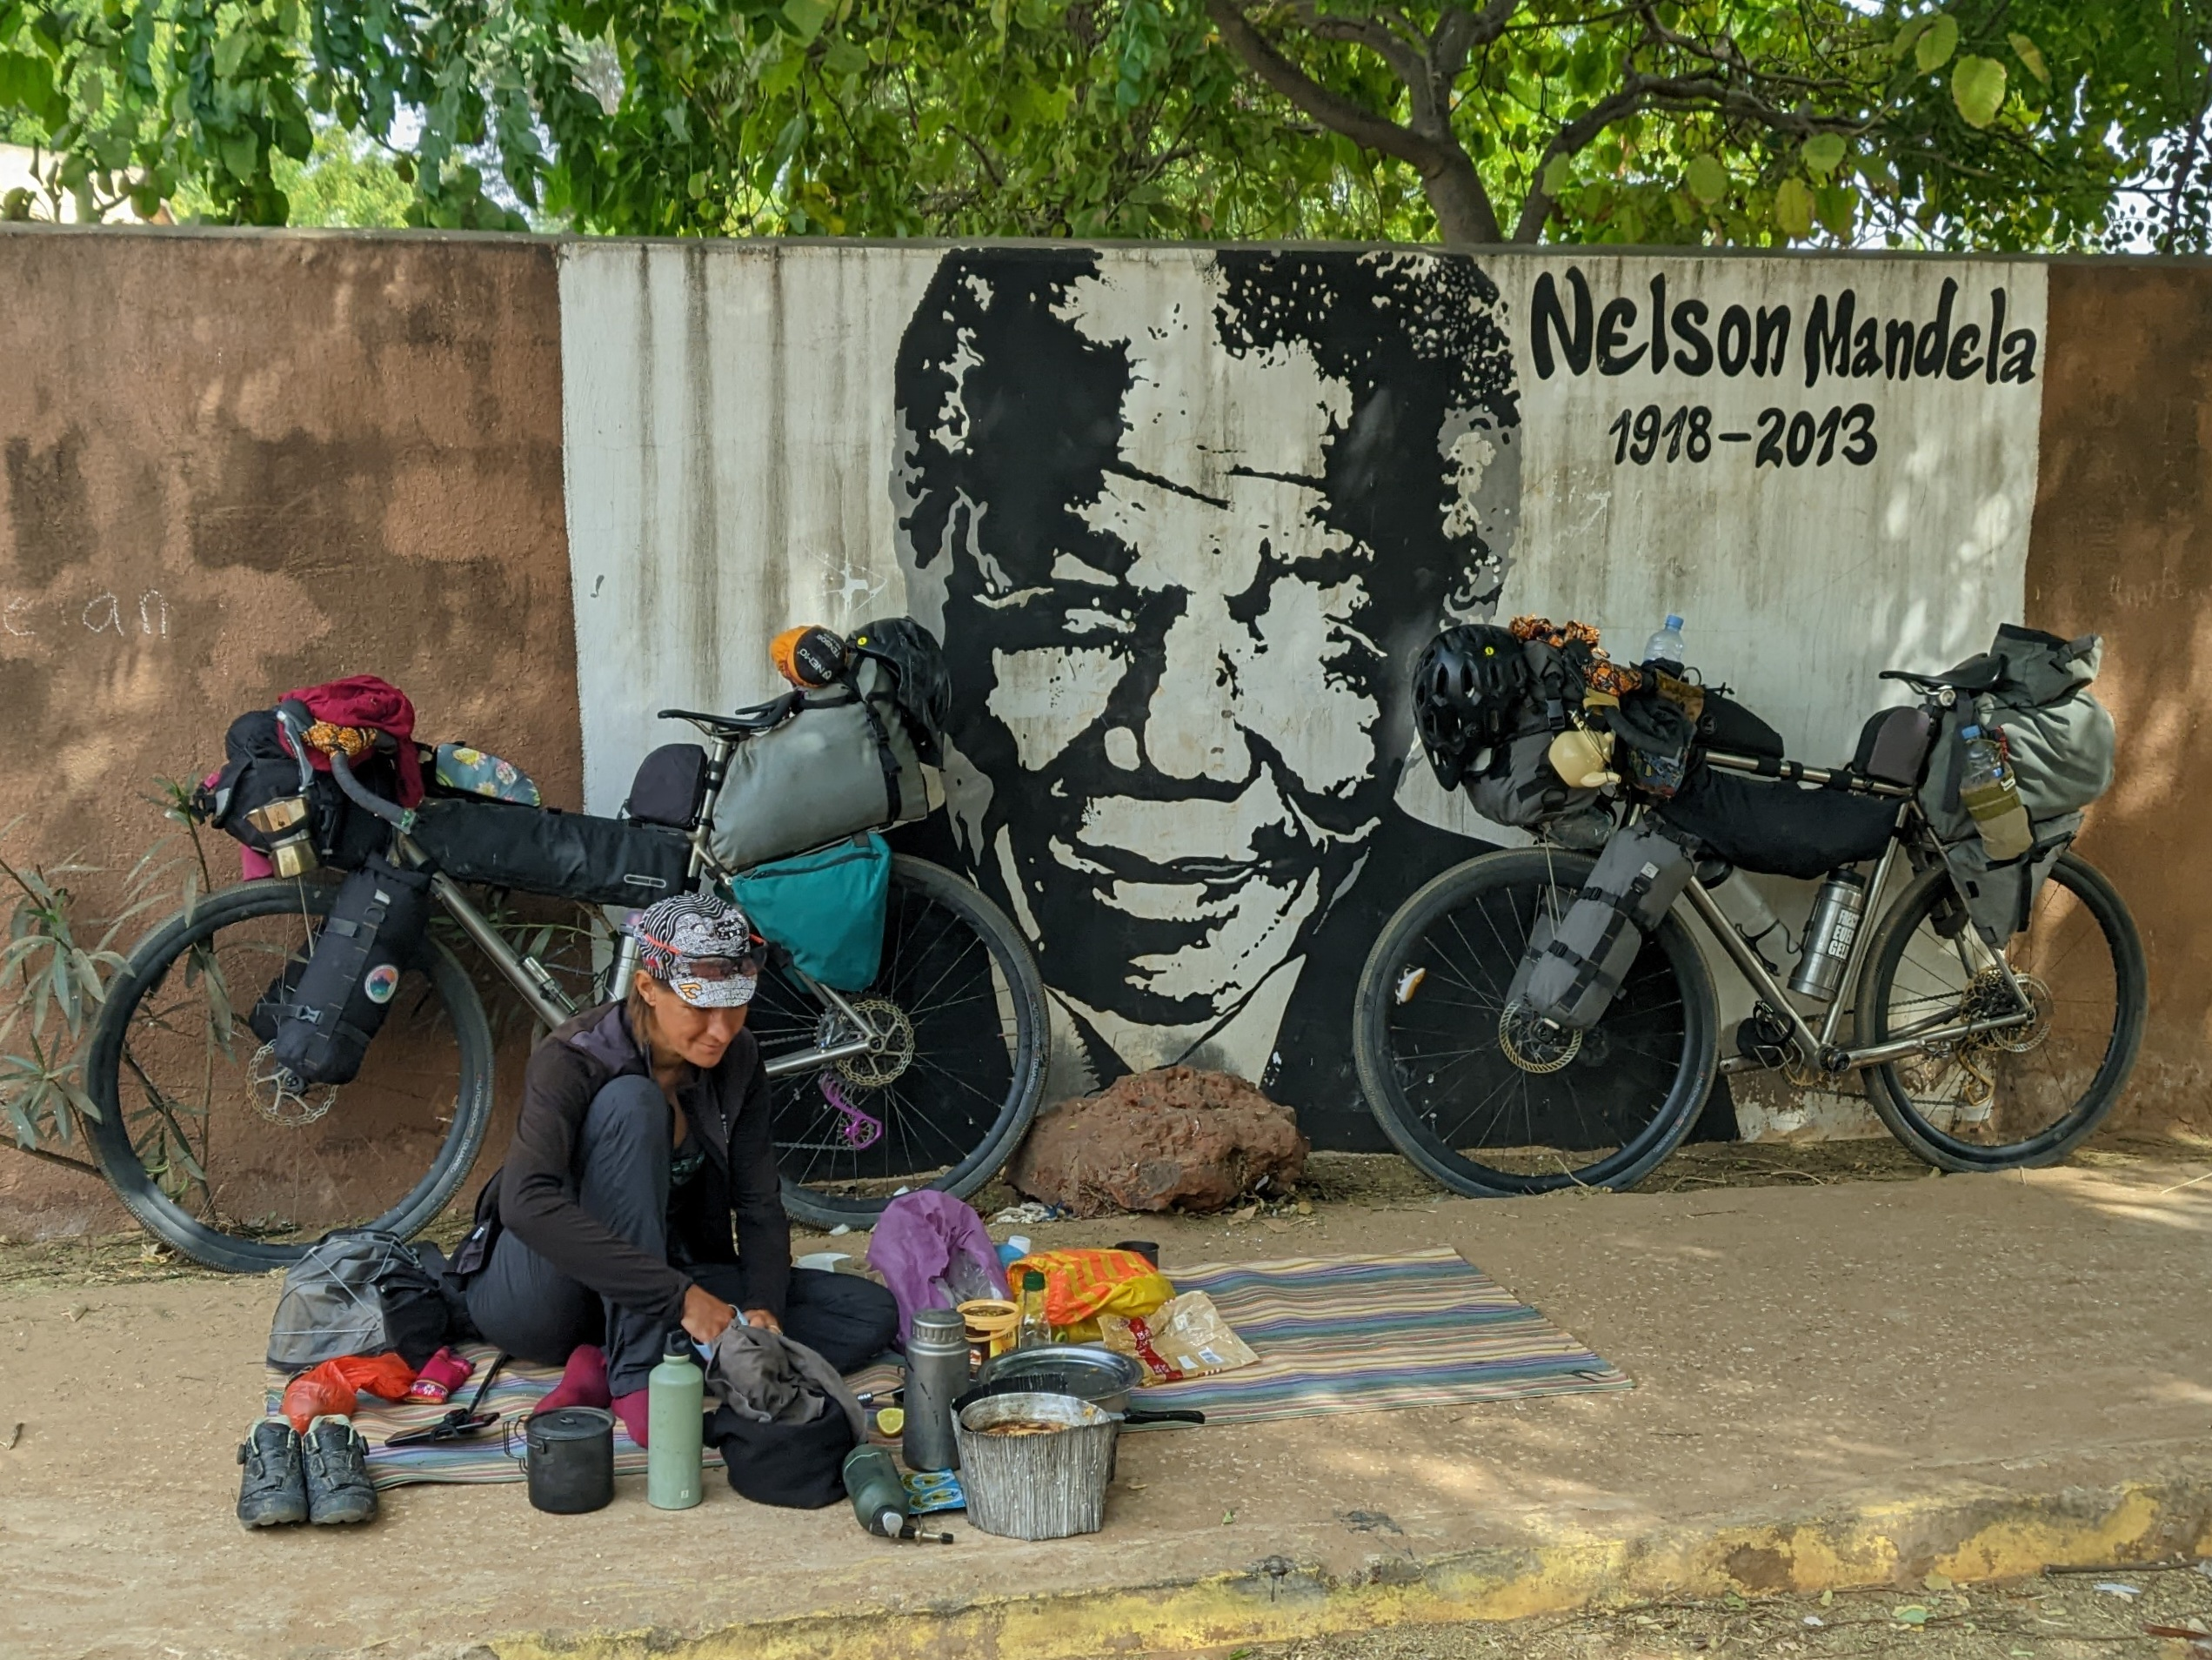
\includegraphics[width=0.5\textwidth,height=\textheight]{../pics/001/Cooking_Senegal_02.jpg}
\includegraphics[width=0.5\textwidth,height=\textheight]{../pics/001/Cooking_Portugal_01.jpg}

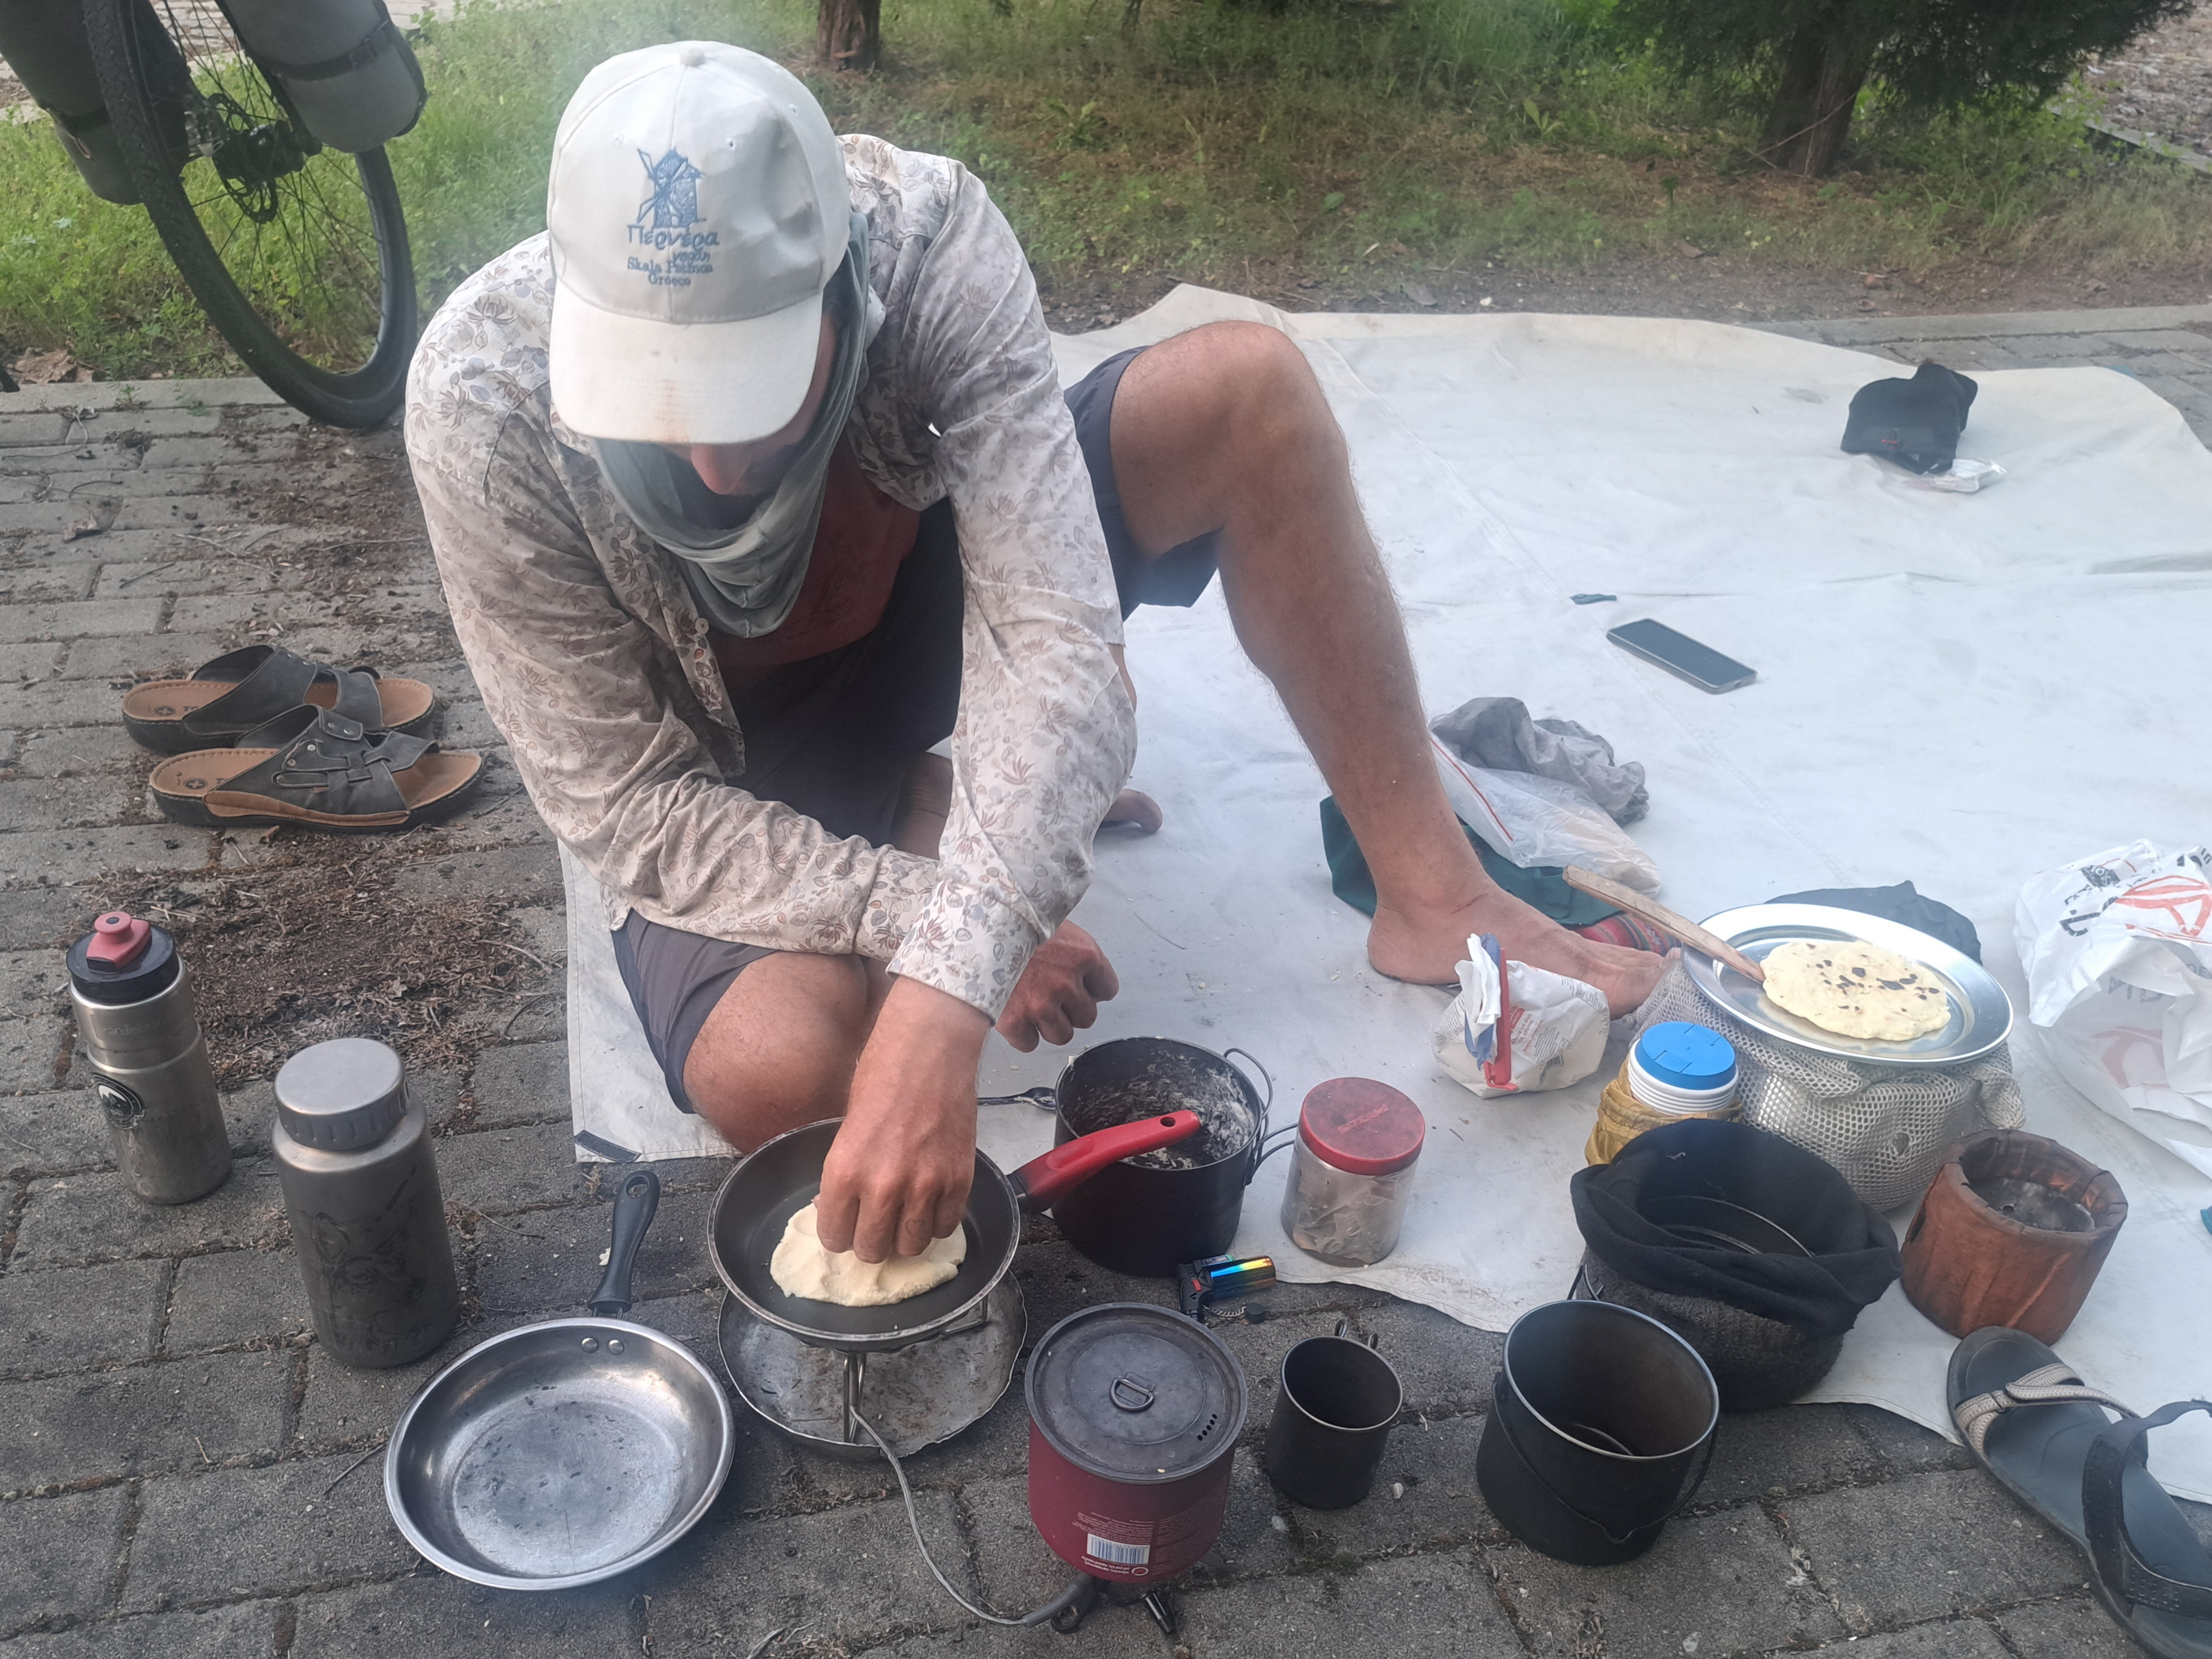
\includegraphics[width=0.5\textwidth,height=\textheight]{../pics/001/Cooking_Bulgaria_01.jpg}
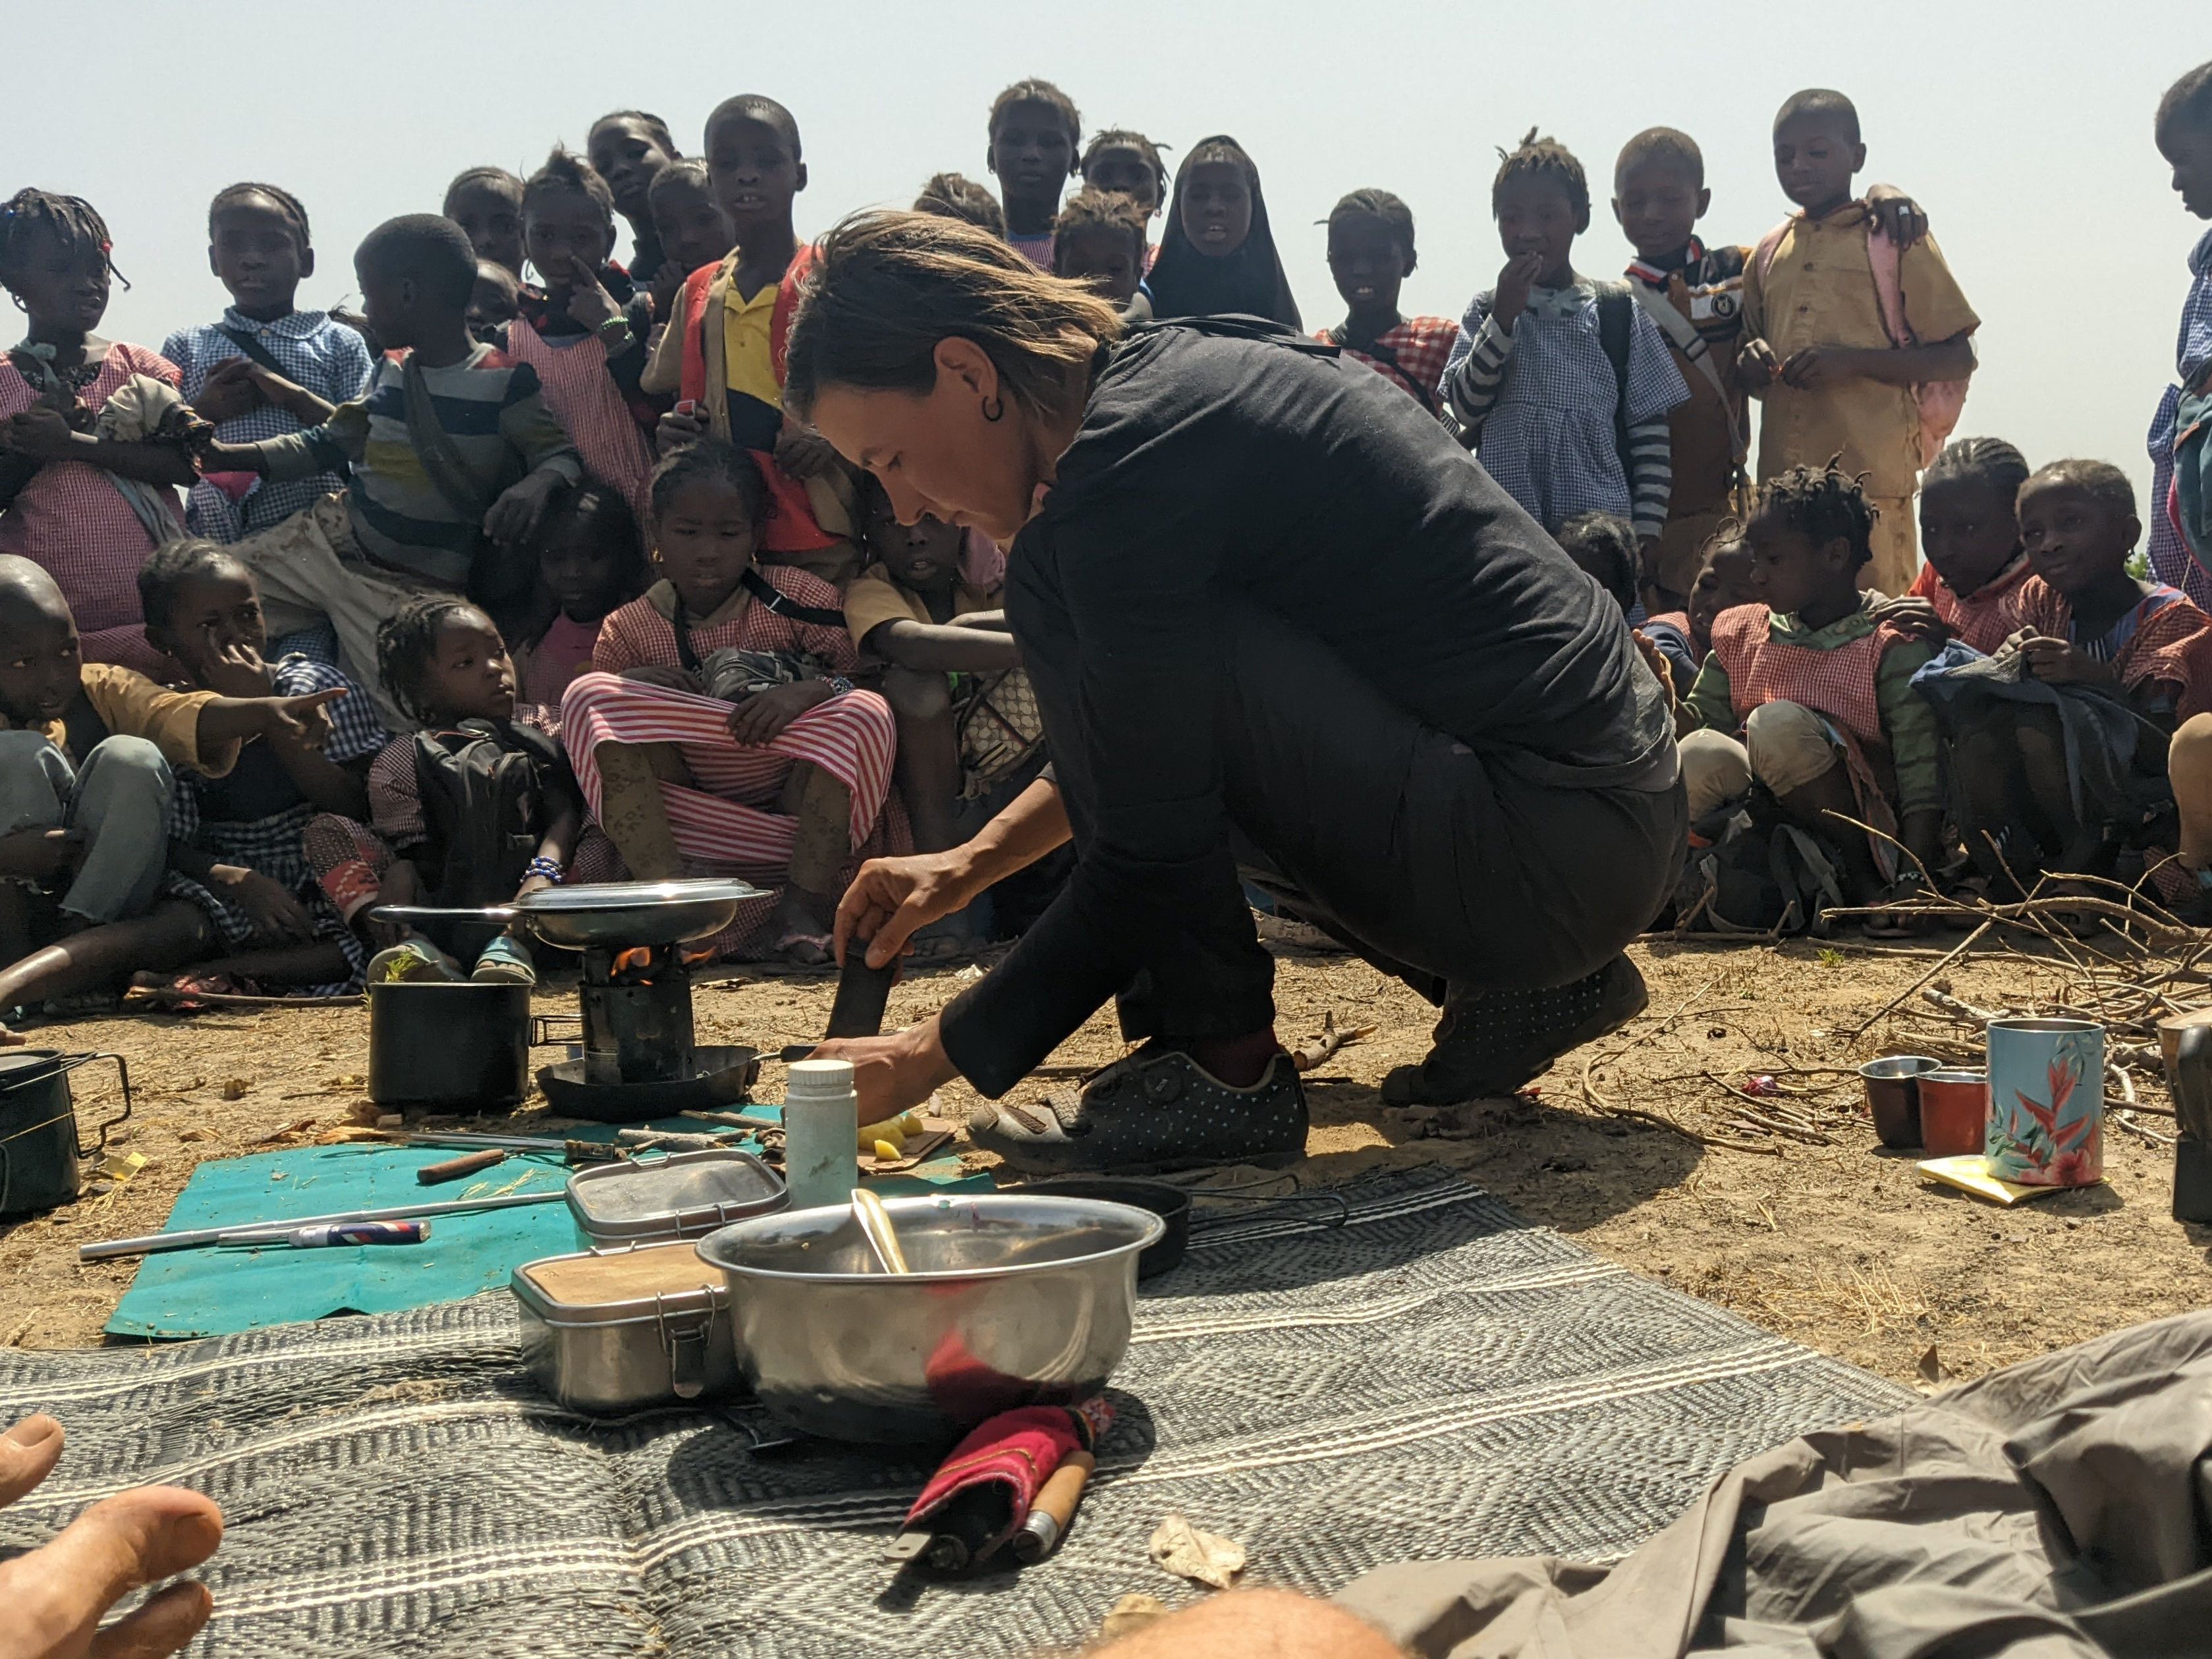
\includegraphics[width=0.5\textwidth,height=\textheight]{../pics/001/Cooking_Senegal_01.jpg}

\includegraphics[width=0.5\textwidth,height=\textheight]{../pics/001/Hotel_Roof_01.jpg}
\includegraphics[width=0.5\textwidth,height=\textheight]{../pics/001/Hotel_Room_01.jpg}

\textbf{Topleft:} Cooking pancakes next to the road in Senegal.
\textbf{Topright:} Cooking in Portugal.

\textbf{Middleleft:} Cooking on a parking lot in Bulgaria.
\textbf{Middleright:} Cooking with spectactors in Westafrica.

\textbf{Downleft:} Cooking on hotelroof in Iran. \textbf{Downright:}
Boiling coffee in hotel bathroom (Iran). \newpage

\section{Credit}\label{credit}

It took me quite a while to collect all this information and compile it
into this e-book. Knowledge must be freely accessible to everyone, you
can read and download this for free. However, it makes sense to donate
some money (either cryptocurrency or fiat) as a sign of appreciation and
respect.

--

Iban €: GB27 REVO 0099 7077 9493 72 Swift: REVOGB21

Iban CHF/\$: CH53 0630 0336 7809 4056 4 Swift: VABECH22

Revolut: (\textbf{brandisbrand?})

Paypal: boost@brandisbrandisbrand.com

BTC: bc1qpfljs02fmad7575fs2skjz5u02plzqw0g3xt6d

ETH: 0x4a92a90C22b78Cbf8672a12A0BB88983bA77fe3a

--

\end{document}
